\begin{figure}[H]
    \centering
    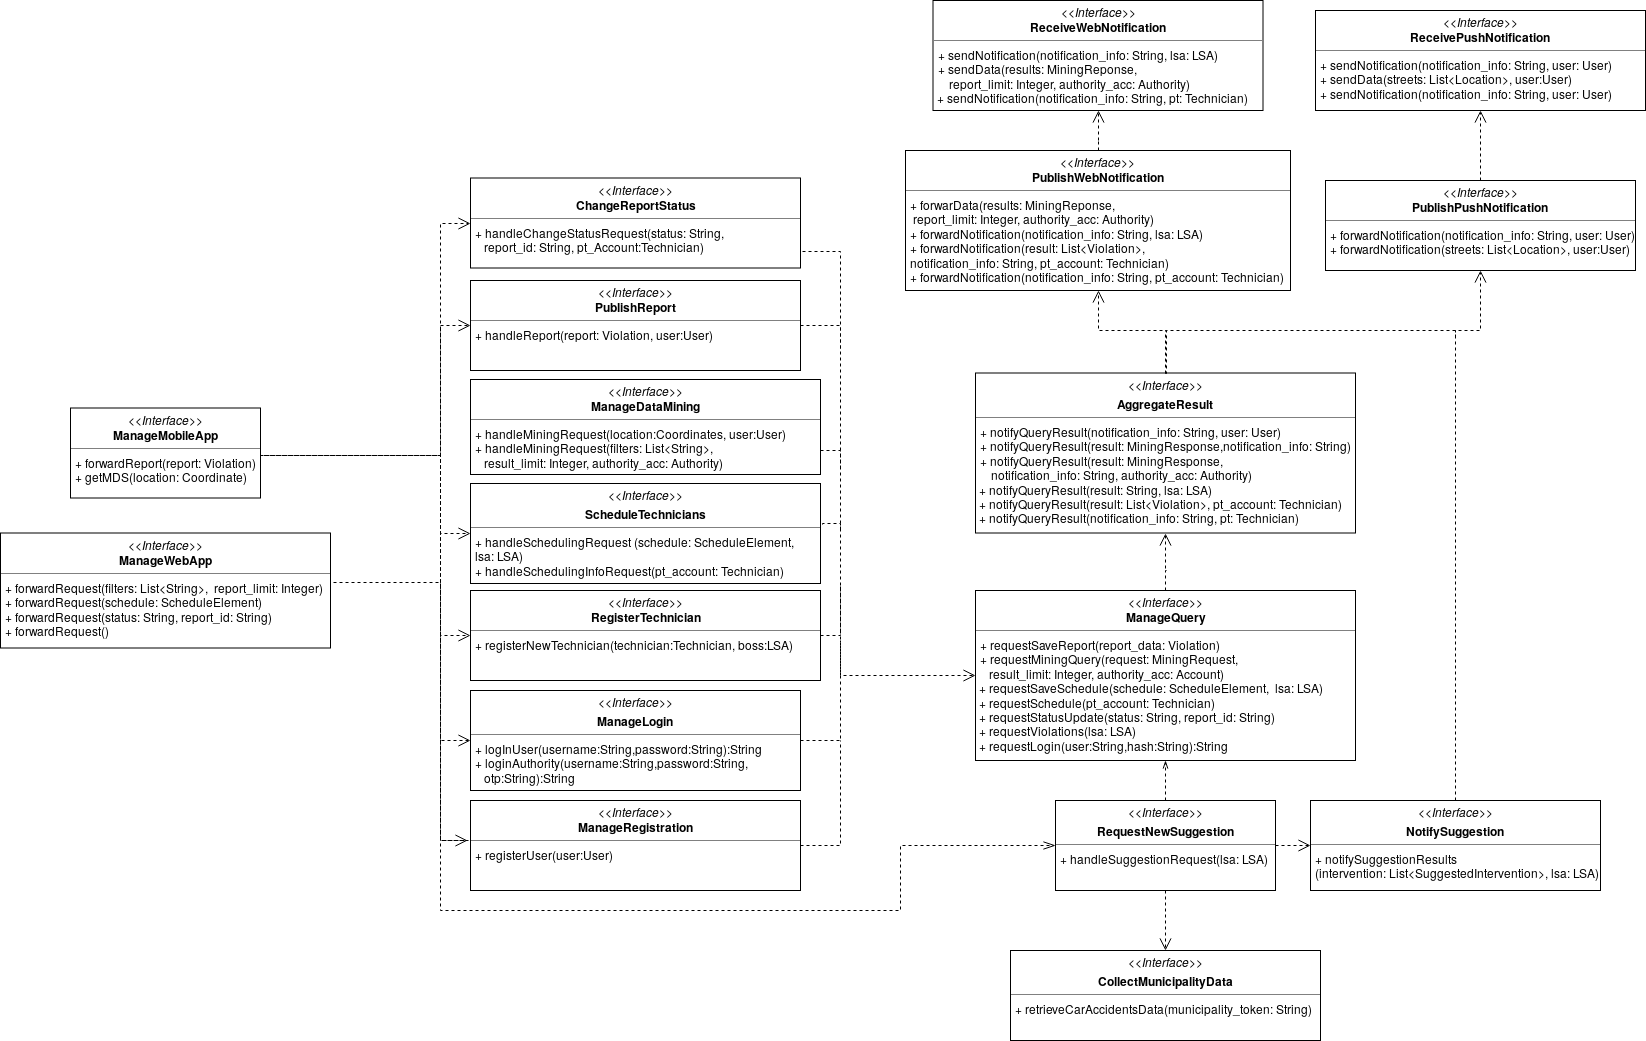
\includegraphics[width=1.1\textwidth]{UML_diagrams/interface_diagram_safestreets}
    \caption{Interface diagram}
    \label{fig:interface_diagram}
\end{figure}
In the figure \ref{fig:interface_diagram} the component interfaces belonging to the application server are represented with respect to what was shown in the Component diagram. The arrows represent dependency relations and depict the dependency tree of the application backend interfaces. 
The functions represented in the interface diagram have the following properties:
\begin{itemize}
    \item The signature of this functions are built only for conceptual showing purposes and they might differ in the final implementation;
    \item The main part of this diagram's functions have been pictured for guaranteeing a correct correspondency with the sequence diagrams of the previous paragraph, therefore some functions are submitted to the overloading technique;
    \item They are offered by the application backend component to one another or to other SafeStreets system components (mobile application and web application).
\end{itemize} 
In order to better understand how the interfaces work and how they are correlated, the following list of clarifications (assumptions) have been considered:
\begin{itemize}
    \item The frontend interfaces have been generically represented by the ReceivePushNotification and ReceiveWebNotification interfaces for dependency purposes. For the sake of simplicity, they have not been analyzed in depth as it is not relevant for the system global functioning;
    \item The workflow of the operation of the SafeStreets system is the following:
        \begin{itemize}
            \item In order to perform any of the functionalities offered by the application backend, the external applications interacts to the ManageMobileApp and ManageWebApp by a RESTful API service;
            \item The functions of these two interfaces forward the requests to the interface of the component related to the called API, propagating also all the parameters embedded to the request (if correctly formalized);
            \item When one of its function is called, the interface of the target component takes in charge the request and let the component do its computation;
            \item Once computation is done, the ManageQuery interface is called in order to interact with the database;
            \item At this point, the component related to the ManageQuery interface execute all the necessary queries and directly forwards the results to the AggregateResult interface;
            \item In this component, the result of the computation is formalized and forwarded to the PublishWebNotification interface in case the request came from a web application (LSA or Technician accounts) or from a mobile application (User)\textsuperscript{[1]};
            \item The publishing interfaces collect the responses and forward them to the devices that performed the operation\textsuperscript{[2]};
            \item The ReceiveWebNotification and ReceivePushNotification API interfaces receive asynchronously the responses and let the local applications handle them.
        \end{itemize}
    It is paramount to underline that the workflow of operations cannot be traversed in the opposite way. For this reason, all interface functions does not have a return type;
    \item The calls of the interfaces functions are performed synchronously: as explained at the previous point, the system operations flow only one way and the output of the previous ones is piped as input to the next one. Without a synchronous function calling system, the piping could not be implemented;
    \item The ManageQuery interface's functions don't have a queryType parameter because it can be inferred from the parameters of the functions: the requestMiningQuery function can be univocally inferred as a SELECT request, the requestSaveSchedule can be univocally inferred as an INSERT and so on;
    \item The ManageQuery interface is the only interface that leads to the QueryManager component. Therefore, all of the previous interfaces depend on it for query executions;
    \item The LoginManager's functions are the only ones that return a value (String): this is due to the authentication token, which has to be backpropagated to the URIManager component in order to perform its functions.
\end{itemize}
\textbf{\textsuperscript{[1]}}: all of the functions of the interfaces that requires a response have the submitter's account as a parameter: this is both necessary for the specific computation of the offered functions and for mapping the response to the submitter. If in some cases the account is not explicitly specified, it is because it can be retrieved by other parameters (e.g. requestSaveReport: the submitter is the violation.user).\newline
\textbf{\textsuperscript{[2]}}: the SafeStreets system handles a table with <Account, Address> tuples, which allows the Notification Service components to forward the results of computation.
\begin{figure}[H]
    \centering
    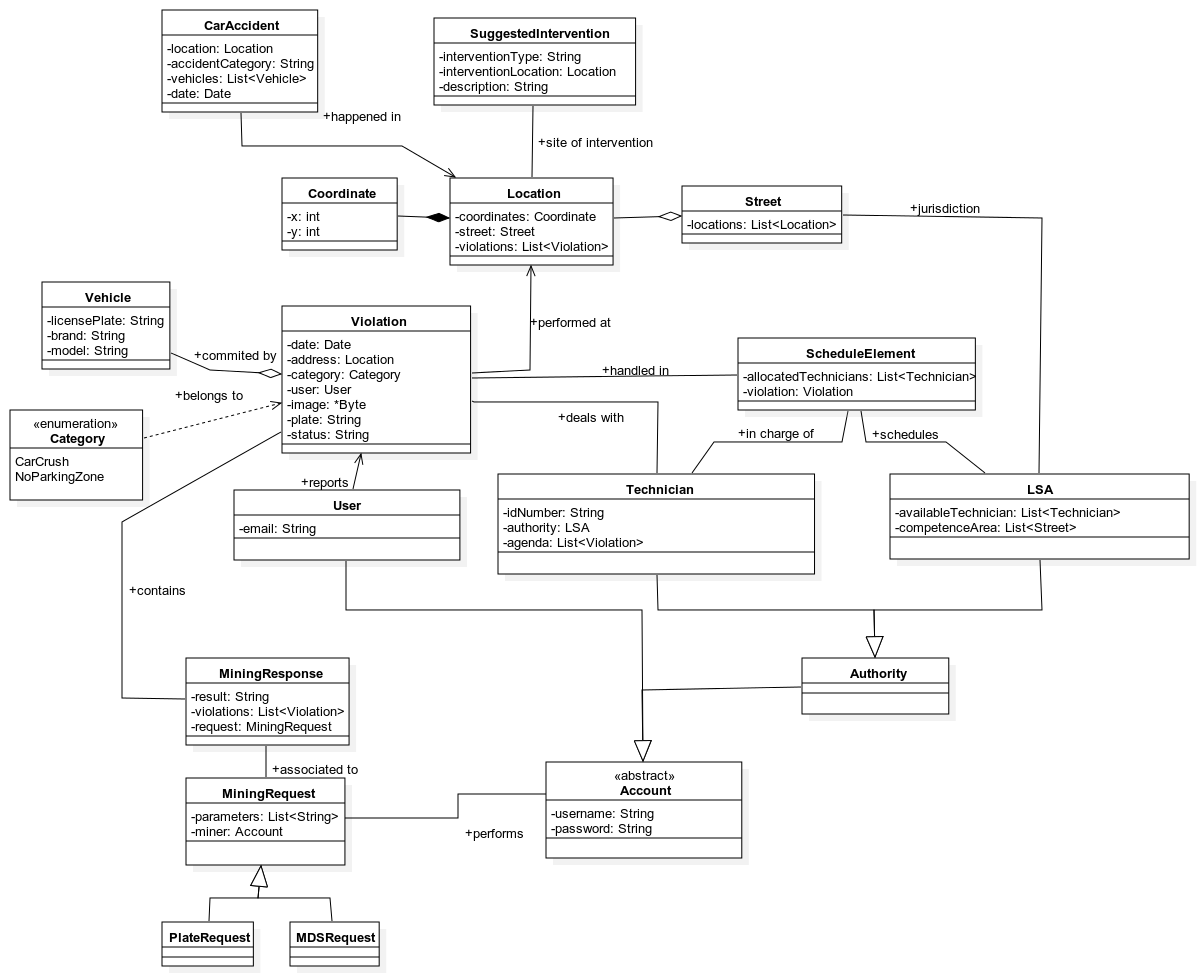
\includegraphics[width=1.1\textwidth]{UML_diagrams/class_diagram_safestreets}
    \caption{Class diagram}
    \label{fig:class_diagram}
\end{figure}
In figure \ref{fig:class_diagram}, the SafeStreets class diagram is represented. This version of the class diagram is similar to the one present in the RASD document, a part from:
\begin{itemize}
    \item The Mining request generalization, in order to add a new useful and extendible design pattern;
    \item The ScheduleElement class, which represents the n-n relation between Technicians and Violations: instead of representing this multiple relation in a singleton class which associate Technicians and Violations, the ScheduleElement objects represent tuples that links a single violation to many Technicians ($\le 5$ as stated in the RASD document). In this way, the system allows LSAs to schedule many Technicians to a specific violation as pictured in the web application mockups. The opposite operation (Technician to many violation) is not allowed up to this version of the system;
    \item The CarAccident class, which represent the aggregation of a single datum collected from the Municipality information system;
    \item The authority generalization of the classes LSA and Technician, in order to identify those classes of accounts which belongs to authorities, therefore they can perform a series of action which are forbidden to Users. 
\end{itemize}
